\documentclass[12pt]{beamer}
\usepackage{color}
\usepackage{xcolor}
\usepackage{amsmath}
\usepackage[labelfont=bf]{caption}
\usepackage{graphicx}  %package graphic
\usepackage{tikz}
\usetikzlibrary{shapes}
\usepackage{subcaption}
\usetikzlibrary{automata, positioning, arrows}
\usetheme{Boadilla}   
\usepackage{xeCJK}
\usepackage{stmaryrd}
\usepackage{adjustbox}

\begin{document}
\begin{frame}{Illustration of $\mathcal{F}_{\phi}$}
	\tikzset{
		%->, % makes the edges directed
		every cross out node/.append style={-,solid},
		>=stealth, % makes the arrow heads bold
		every edge/.style={draw, thick, black},
		node distance=0.8cm and 2.3cm, % specifies the minimum distance between two nodes. Change if necessary.
		every state/.style={thick, fill=gray!10, scale = 0.6}, % sets the properties for each ’state’ node
		initial text=$ $, % sets the text that appears on the start arrow
		}
	\begin{figure}[ht]
		\centering
		\begin{tikzpicture}
			\node[state, initial] (ini) at (-5, 0) {};
			\node[state, accepting] (last) at (5, 0) {};

			\node[state] (t2) at (-2, 2) {t2};
			\node[state] (t1) at (-3.6, 2) {t1};
			\node[state, accepting] (t3) at (-2.8, 3.2) {t3};

			\node[state] (t4) at (2, 2) {t4};
			\node[state, accepting] (t5) at (3.6, 2) {t5};
			\node[state] (t6) at (2.8, 3.2) {t6};

			\node[state, accepting] (b2) at (-2, -2) {b2};
			\node[state] (b1) at (-3.6, -2) {b1};
			\node[state] (b3) at (-2.8, -3.2) {b3};

			\node[state] (b4) at (2, -2) {b4};
			\node[state] (b5) at (3.6, -2) {b5};
			\node[state] (b6) at (2.8, -3.2) {b6};

			\node[state, accepting] (b7) at (0, -2.5) {b7};

			\draw (ini) edge[->, bend left = 20] (t1);
			\draw (t1) edge[->, bend right = 20] (t2);
			\draw (t2) edge[->, bend right = 20] (t3);
			\draw (t3) edge[->, bend right = 20] (t1);
			\draw (t2) edge[->, bend left = 20] (t4);
			\draw (t4) edge[->, bend right = 20] (t5);
			\draw (t5) edge[->, bend right = 20] (t6);
			\draw (t6) edge[->, bend right = 20] (t4);
			\draw (t5) edge[->, bend left = 20] (last);

			\draw (ini) edge[->, bend right = 20] (b1);
			\draw (b1) edge[->, bend left = 20] (b2);
			\draw (b2) edge[->, bend left = 20] (b3);
			\draw (b3) edge[->, bend left = 20] (b1);
			\draw (b2) edge[->, bend right = 20] (b7);
			\draw (b7) edge[->, bend right = 20] (b4);
			\draw (b4) edge[->, bend left = 20] (b5);
			\draw (b5) edge[->, bend left = 20] (b6);
			\draw (b6) edge[->, bend left = 20] (b4);
			\draw (b5) edge[->, bend right = 20] (last);

			\only<2->{
				\tikzset{
					every state/.style={thick, fill=red!50, scale = 0.6}
				}
			}
			\only<2-5>{
				\node[state, accepting] (t3) at (-2.8, 3.2) {t3};
				\node[state, accepting] (t5) at (3.6, 2) {t5};
				\node[state, accepting] (b2) at (-2, -2) {b2};
				\node[state, accepting] (b7) at (0, -2.5) {b7};
			}

			\only<3-5,7-8>{
				\node[state] (b1) at (-3.6, -2) {b1};
				\node[state] (t2) at (-2, 2) {t2};
				\node[state] (t4) at (2, 2) {t4};
			}

			\only<4-5,8>{
				\node[state, initial] (ini) at (-5, 0) {};
				\node[state] (t1) at (-3.6, 2) {t1};
				\node[state] (t6) at (2.8, 3.2) {t6};
				\node[state] (b3) at (-2.8, -3.2) {b3};
			}

			\only<5->{
				\node[state, accepting, fill=gray!10] (last) at (5, 0) {};
				\node[state, accepting, fill=gray!10] (b7) at (0, -2.5) {b7};
			}

			\only<6->{
				\node[state, accepting] (t3) at (-2.8, 3.2) {t3};
				\node[state, accepting] (t5) at (3.6, 2) {t5};
				\node[state, accepting] (b2) at (-2, -2) {b2};
			}

		  \end{tikzpicture}
		  \caption{Illustration of $\mathcal{F}_{\phi} \equiv \nu \mathnormal{y} \cdot \mu \mathnormal{x} \cdot (\text{Pre}(\mathnormal{x}) \cup (\text{Pre}(\mathnormal{y}) \cap \alpha^{\text{MH}}))$}
	\end{figure}
\end{frame}

\begin{frame}{Illustration of $\mathcal{F}'_{\phi}$}
	\tikzset{
		%->, % makes the edges directed
		every cross out node/.append style={-,solid},
		>=stealth, % makes the arrow heads bold
		every edge/.style={draw, thick, black},
		node distance=0.8cm and 2.3cm, % specifies the minimum distance between two nodes. Change if necessary.
		every state/.style={thick, fill=gray!10, scale = 0.6}, % sets the properties for each ’state’ node
		initial text=$ $, % sets the text that appears on the start arrow
		}
	\begin{figure}[ht]
		\centering
		\begin{tikzpicture}
			\node[state, initial] (ini) at (-5, 0) {};
			\node[state, accepting] (last) at (5, 0) {};

			\node[state] (t2) at (-2, 2) {t2};
			\node[state] (t1) at (-3.6, 2) {t1};
			\node[state, accepting] (t3) at (-2.8, 3.2) {t3};

			\node[state] (t4) at (2, 2) {t4};
			\node[state, accepting] (t5) at (3.6, 2) {t5};
			\node[state] (t6) at (2.8, 3.2) {t6};

			\node[state, accepting] (b2) at (-2, -2) {b2};
			\node[state] (b1) at (-3.6, -2) {b1};
			\node[state] (b3) at (-2.8, -3.2) {b3};

			\node[state] (b4) at (2, -2) {b4};
			\node[state] (b5) at (3.6, -2) {b5};
			\node[state] (b6) at (2.8, -3.2) {b6};

			\node[state, accepting] (b7) at (0, -2.5) {b7};

			\draw (ini) edge[->, bend left = 20] (t1);
			\draw (t1) edge[->, bend right = 20] (t2);
			\draw (t2) edge[->, bend right = 20] (t3);
			\draw (t3) edge[->, bend right = 20] (t1);
			\draw (t2) edge[->, bend left = 20] (t4);
			\draw (t4) edge[->, bend right = 20] (t5);
			\draw (t5) edge[->, bend right = 20] (t6);
			\draw (t6) edge[->, bend right = 20] (t4);
			\draw (t5) edge[->, bend left = 20] (last);

			\draw (ini) edge[->, bend right = 20] (b1);
			\draw (b1) edge[->, bend left = 20] (b2);
			\draw (b2) edge[->, bend left = 20] (b3);
			\draw (b3) edge[->, bend left = 20] (b1);
			\draw (b2) edge[->, bend right = 20] (b7);
			\draw (b7) edge[->, bend right = 20] (b4);
			\draw (b4) edge[->, bend left = 20] (b5);
			\draw (b5) edge[->, bend left = 20] (b6);
			\draw (b6) edge[->, bend left = 20] (b4);
			\draw (b5) edge[->, bend right = 20] (last);

			\only<2->{
				\tikzset{
					every state/.style={thick, fill=red!50, scale = 0.6}
				}
			}
			\only<2-5>{
				\node[state, accepting] (t3) at (-2.8, 3.2) {t3};
				\node[state, accepting] (t5) at (3.6, 2) {t5};
				\node[state, accepting] (b2) at (-2, -2) {b2};
				\node[state, accepting] (b7) at (0, -2.5) {b7};
				\node[state, accepting] (last) at (5, 0) {};
			}

			\only<3-5>{
				\node[state] (t1) at (-3.6, 2) {t1};
				\node[state] (t6) at (2.8, 3.2) {t6};
				\node[state] (b3) at (-2.8, -3.2) {b3};
				\node[state] (b4) at (2, -2) {b4};
			}

			\only<4-5>{
				\node[state] (t2) at (-2, 2) {t2};
				\node[state] (b1) at (-3.6, -2) {b1};
				\node[state] (t4) at (2, 2) {t4};
				\node[state] (b5) at (3.6, -2) {b5};
			}

			\only<5>{
				\node[state] (b6) at (2.8, -3.2) {b6};
			}


		  \end{tikzpicture}
		  \caption{Illustration of $\mathcal{F}'_{\phi} \equiv \nu \mathnormal{y} \cdot \mu \mathnormal{x} \cdot (\text{Post}(\mathnormal{x}) \cup (\text{Post}(\mathnormal{y}) \cap R_{\alpha}))$}
	\end{figure}
\end{frame}

\end{document}